\centering
\begin{tikzpicture}
    \pgfmathsetlengthmacro{\imw}{0.33\linewidth}
    \pgfmathsetlengthmacro{\imws}{0.325\linewidth}

    % First image
    \node[inner sep=0pt] (image1) at (0,0)
        {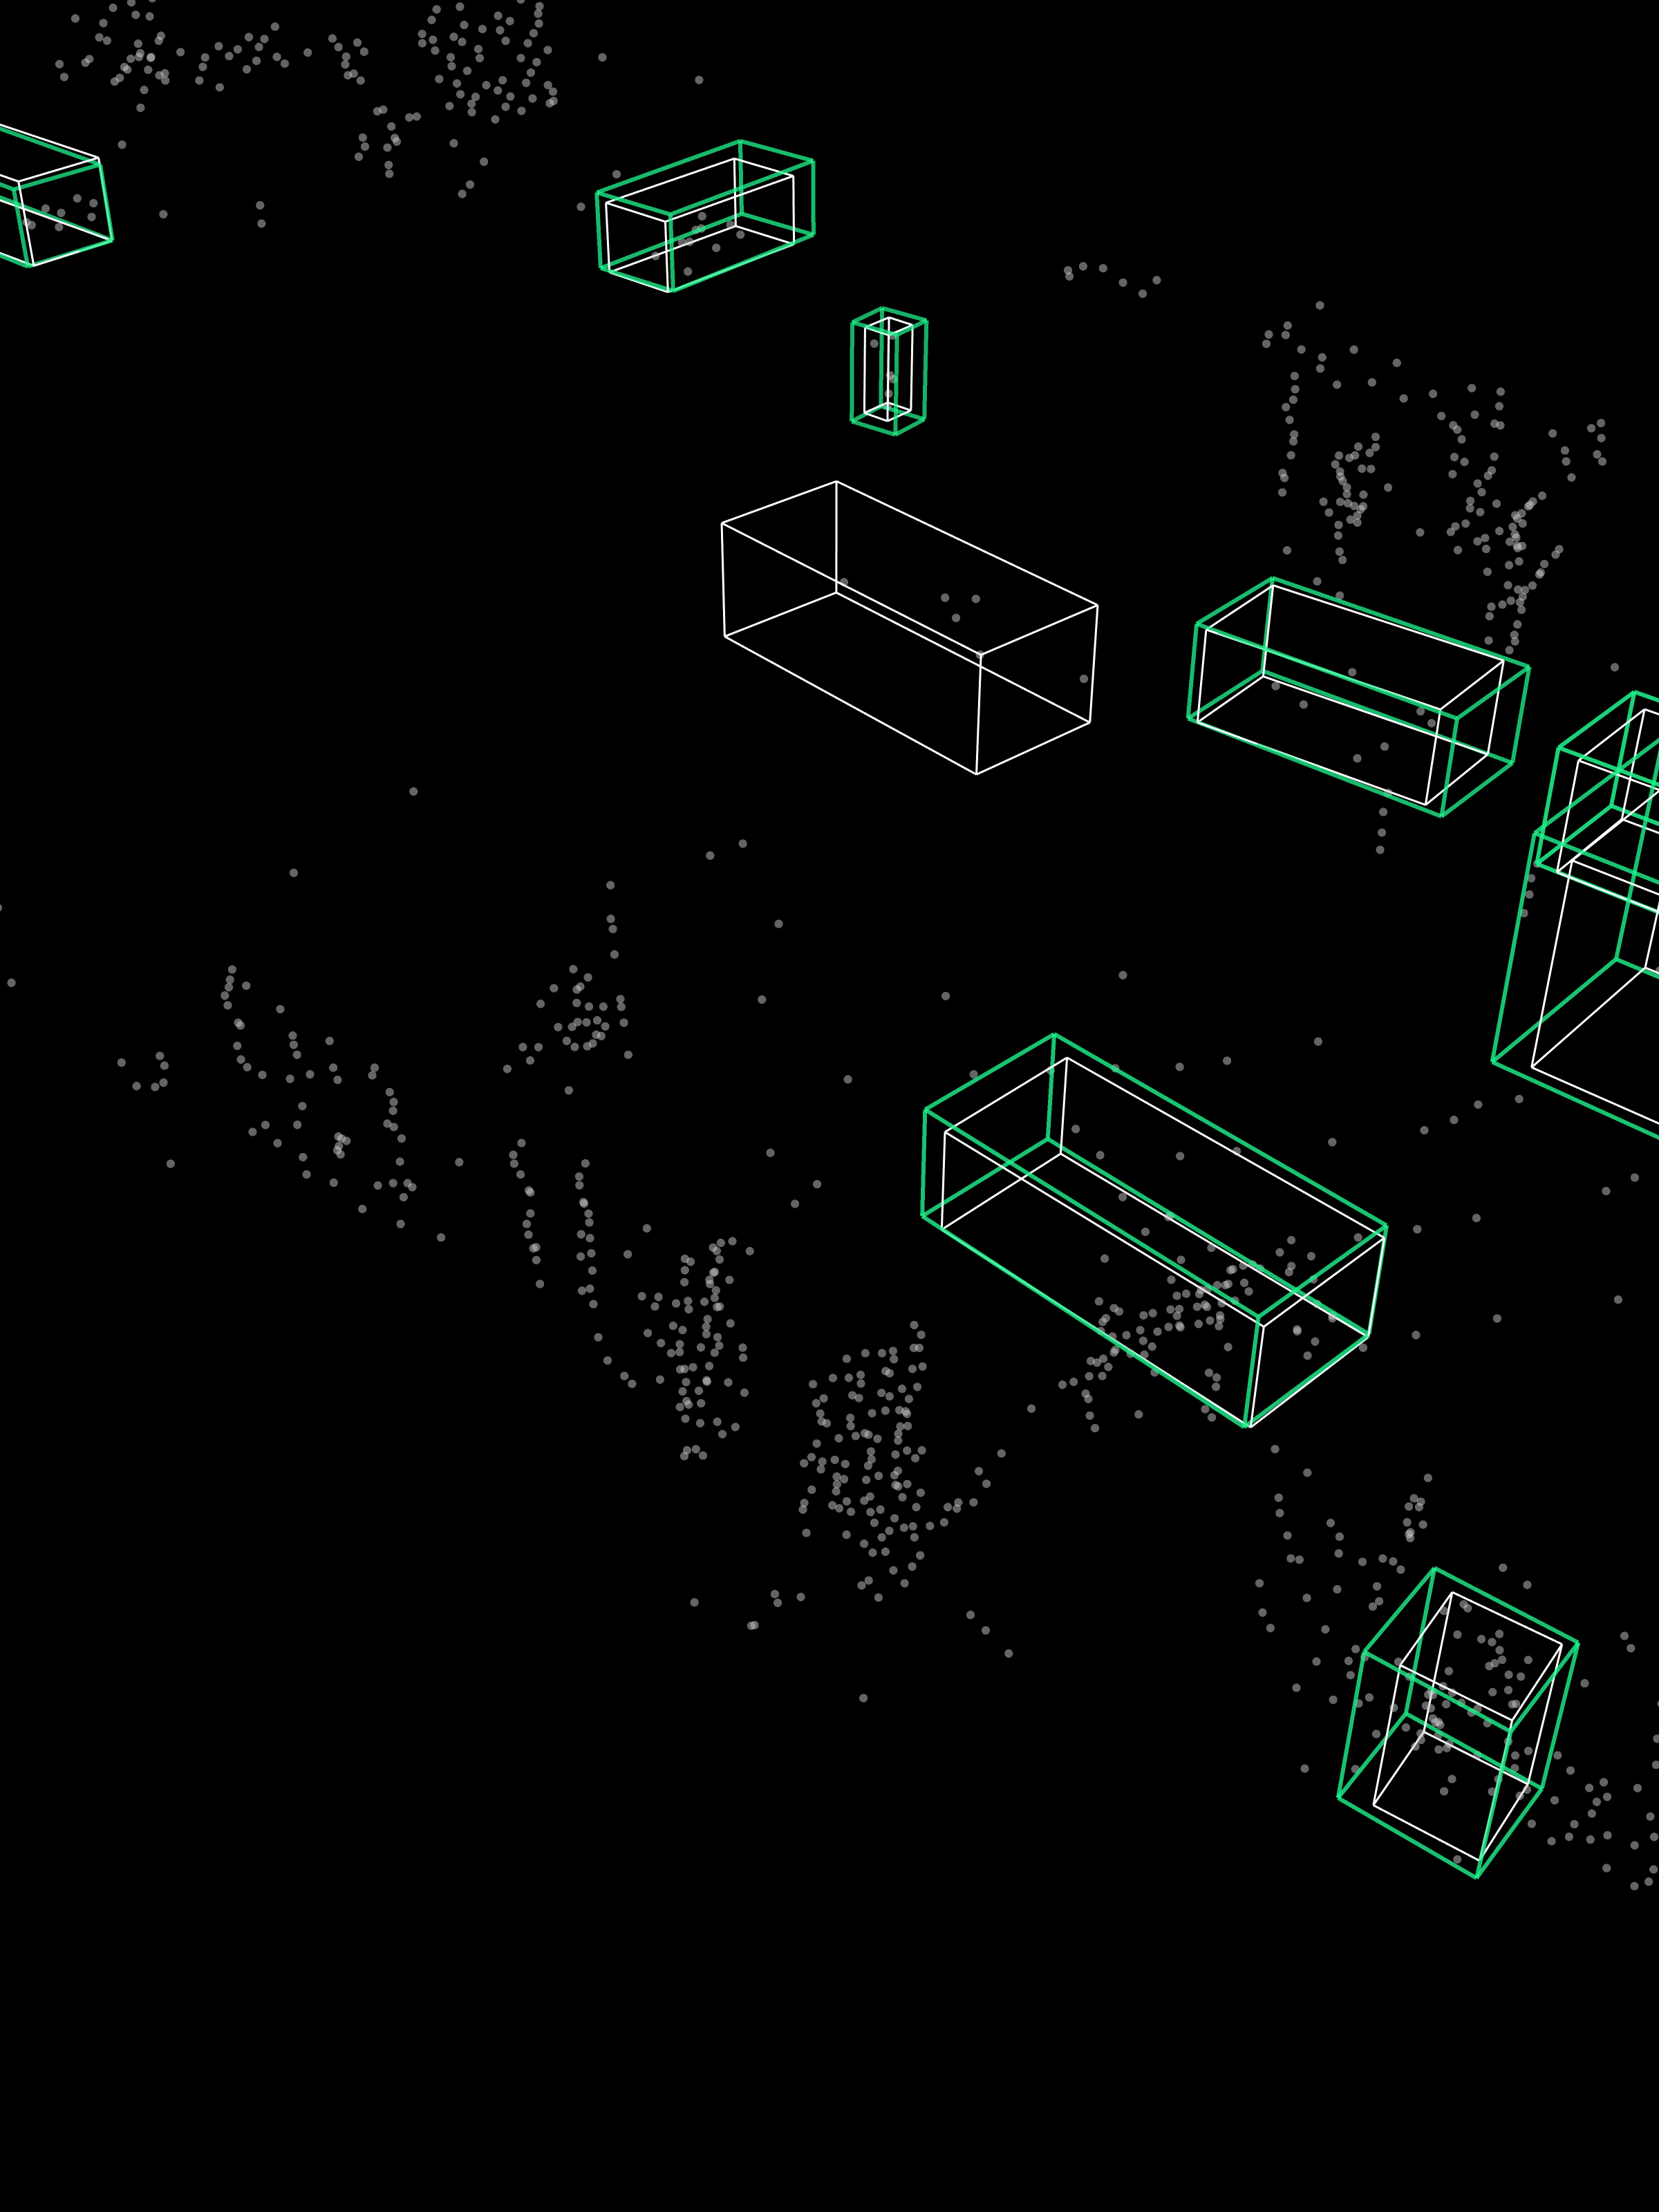
\includegraphics[width=\imw, trim={0cm, 70cm, 0cm, 0cm}, clip]{images/images_for_hook/lidar_proposals_wod_viz_5_198.png}};
    \node[inner sep=0pt, anchor=south, yshift=0.25em] (title1) at (image1.north) {(a) 3D Detector};
    
    % Second image
    \node[inner sep=0pt,anchor=west] (image2) at ($(image1.east)+(0.5em,0em)$)
        {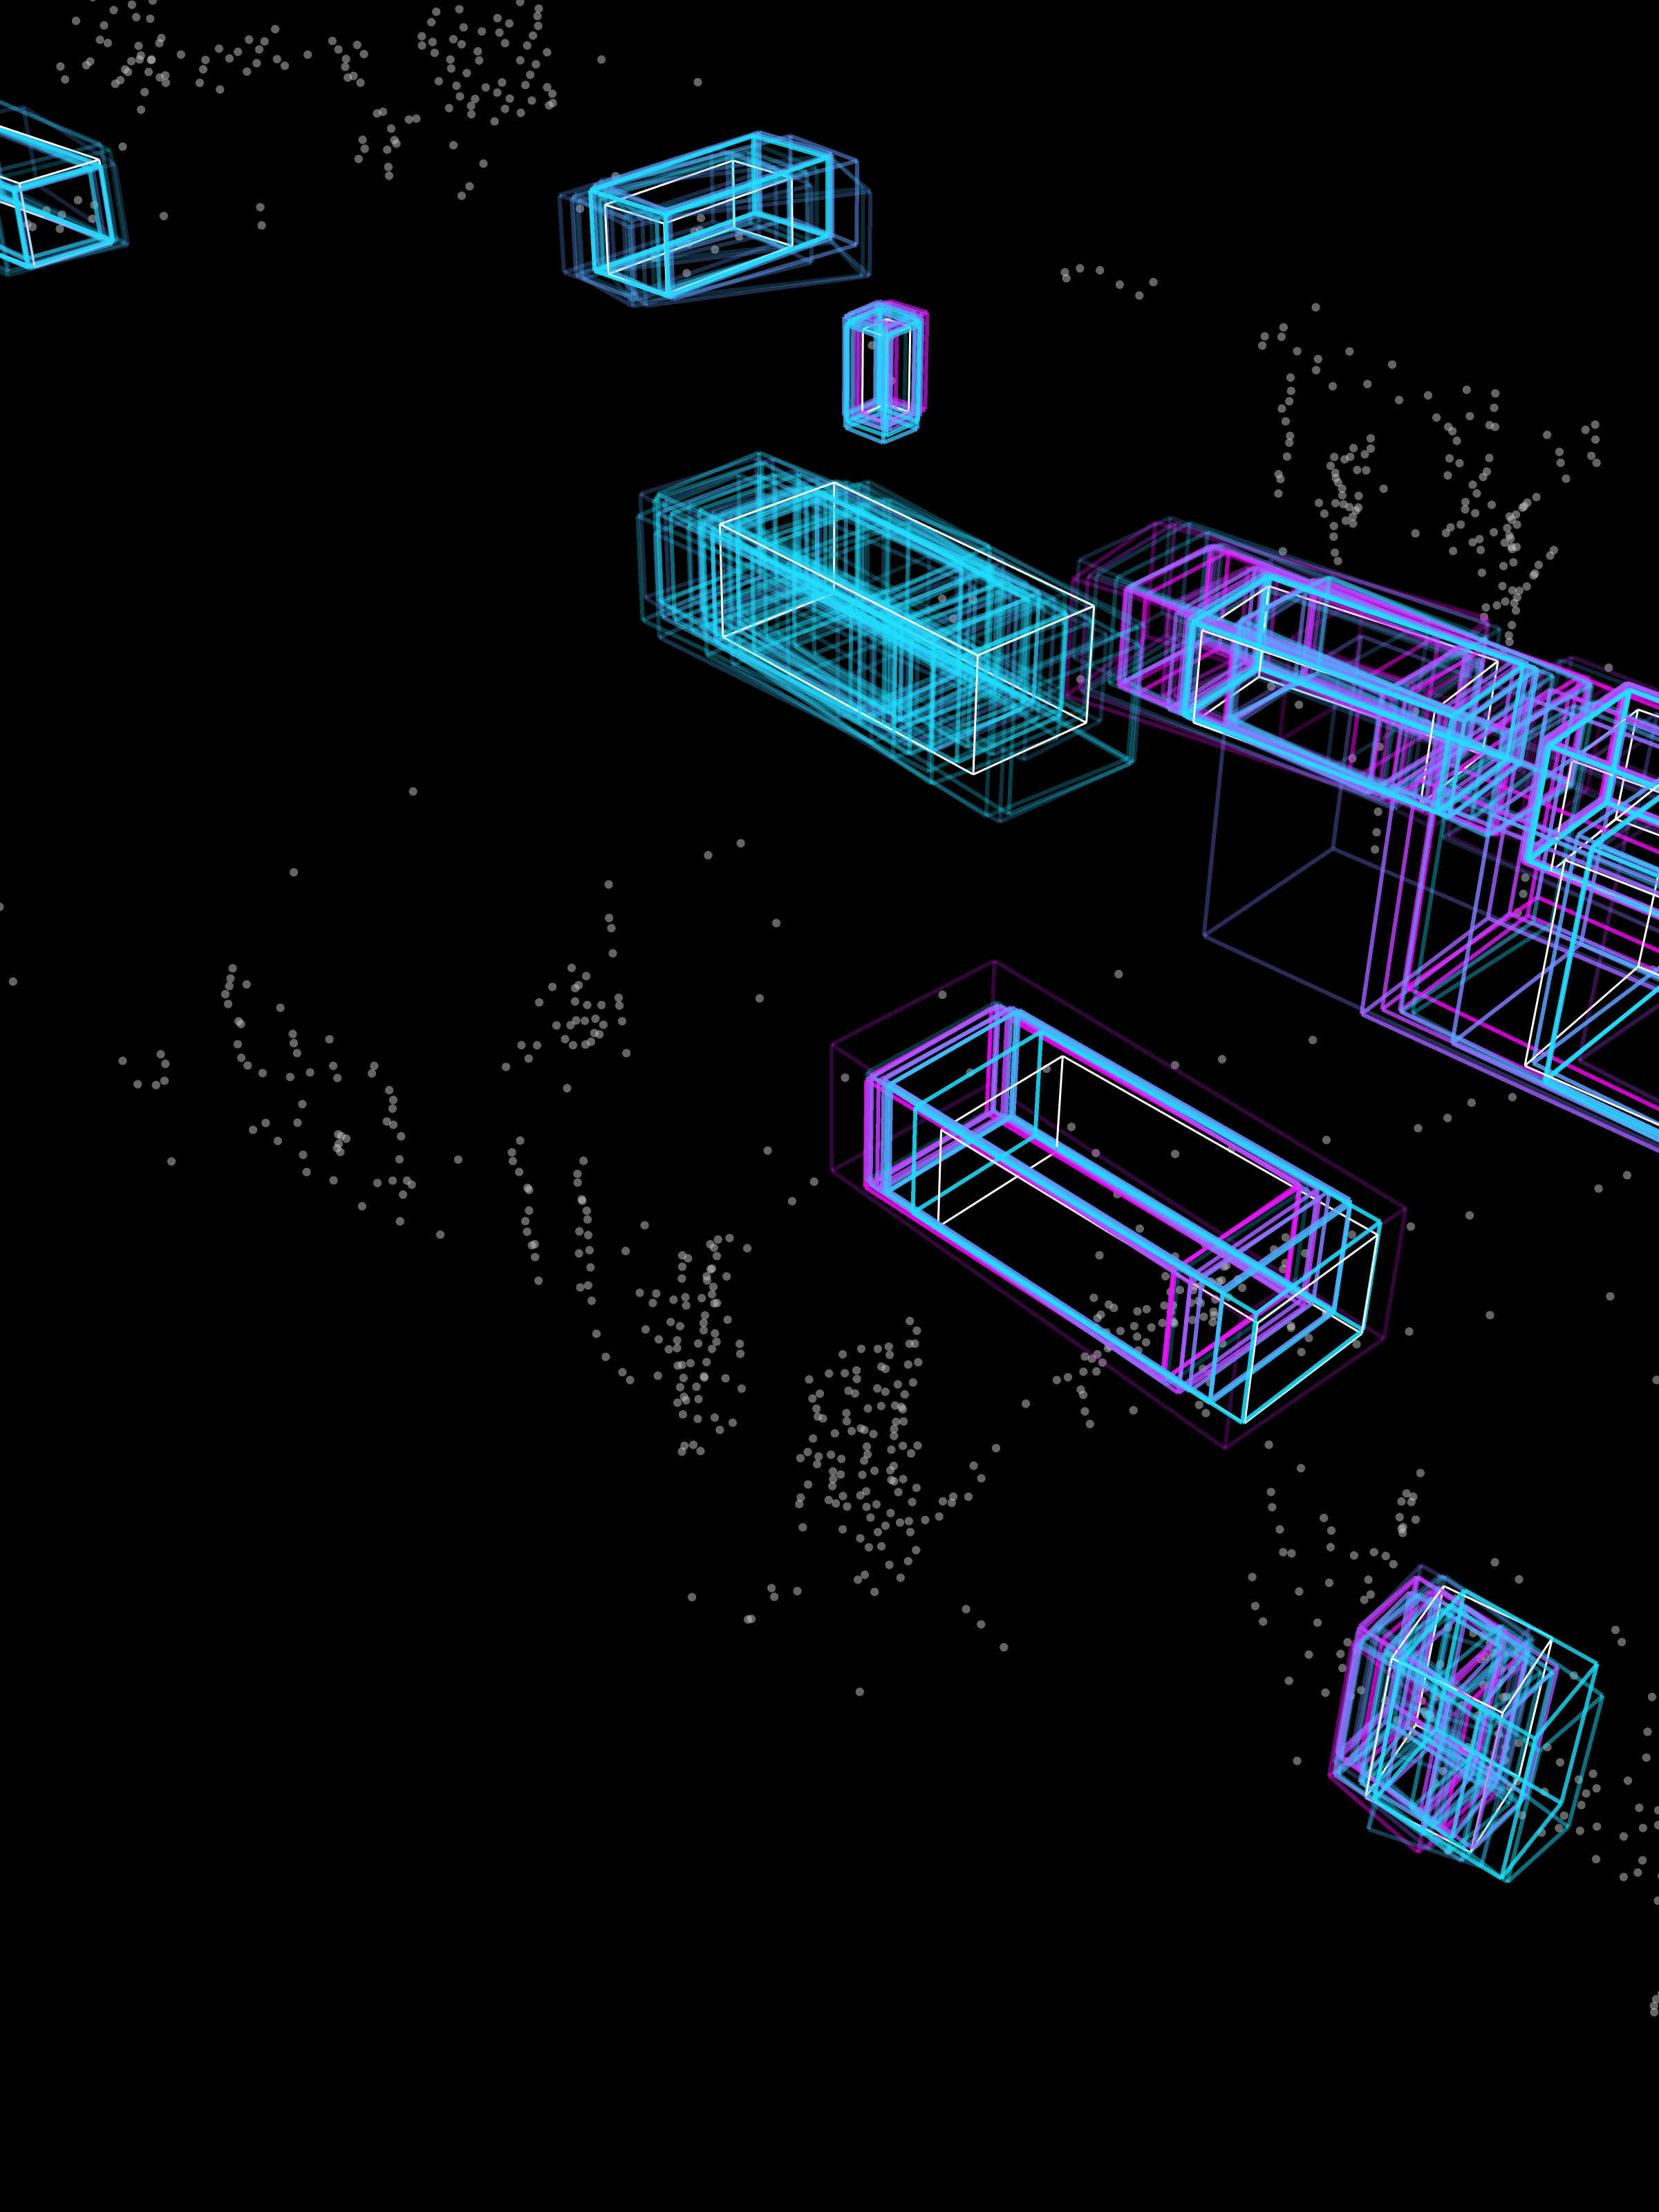
\includegraphics[width=\imw, trim={0cm, 70cm, 0cm, 0cm}, clip]{images/images_for_hook/memory_proposals_wod_viz_5_198.png}};
    \node[inner sep=0pt,anchor=south, yshift=0.25em] (title2) at (image2.north) {(b) Object Memory};
    
    % Third image
    \node[inner sep=0pt,anchor=west] (image3) at ($(image2.east)+(0.05em,0)$)
        {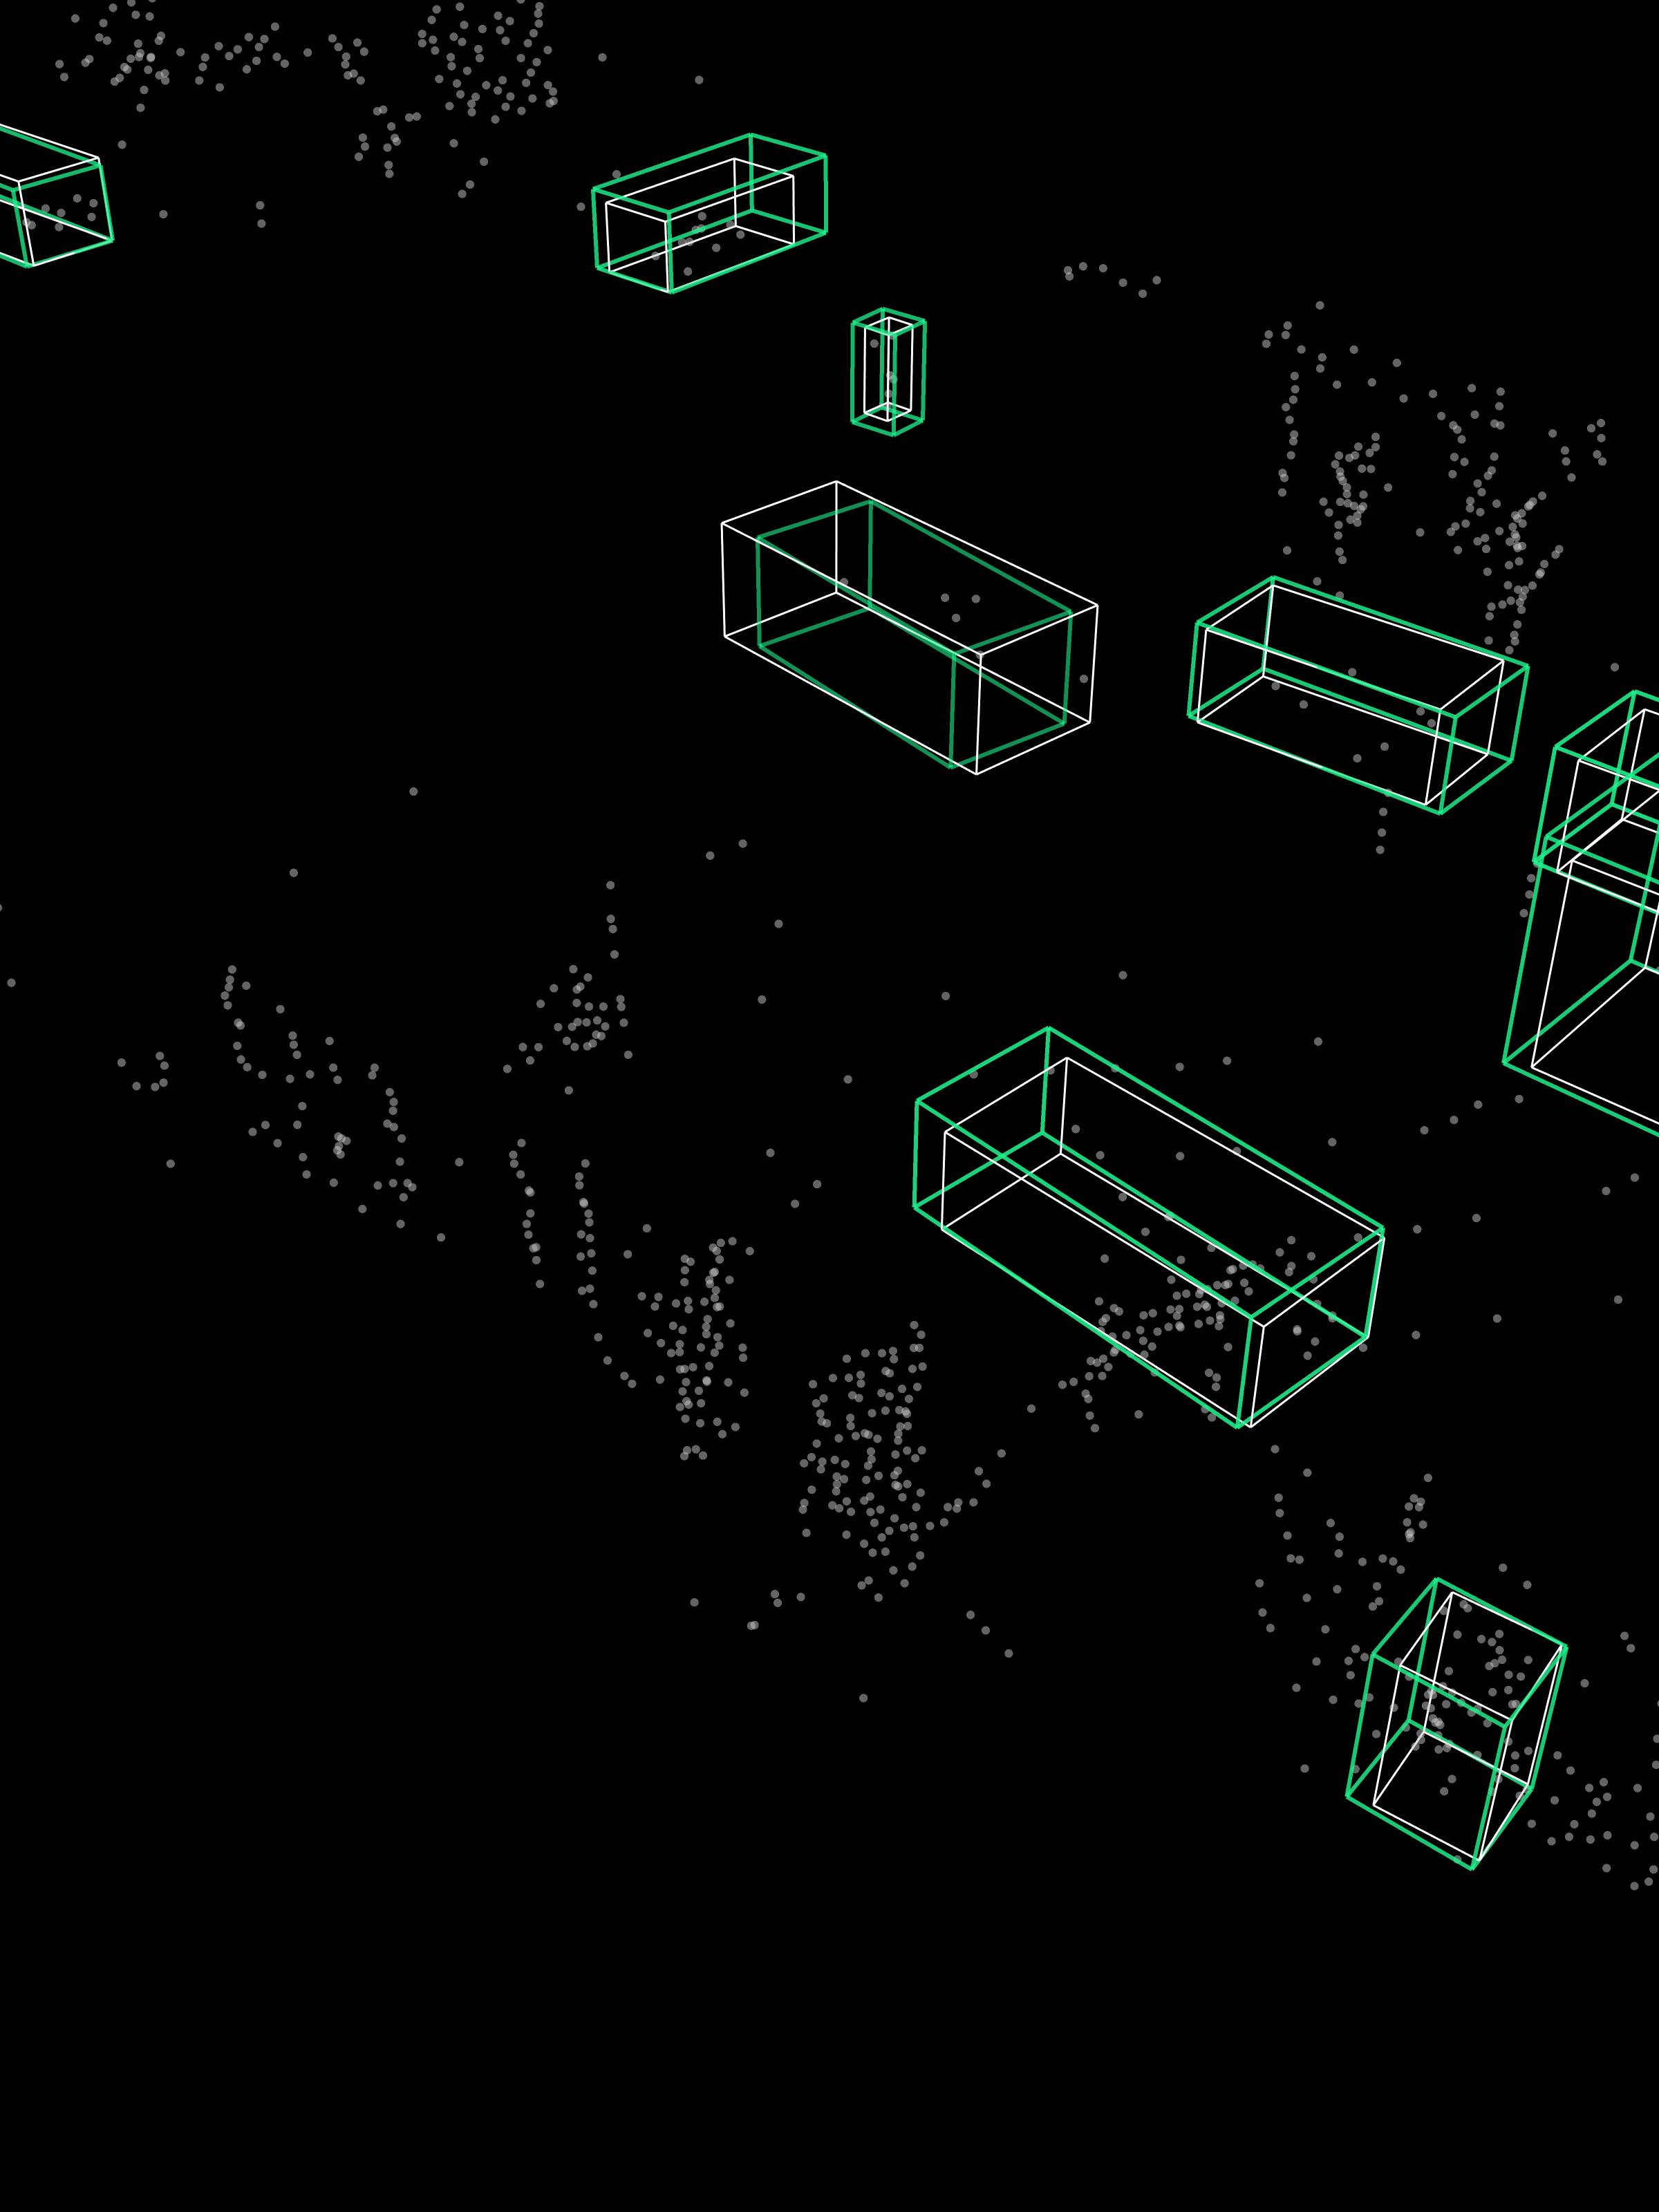
\includegraphics[width=\imw, trim={0cm, 70cm, 0cm, 0cm}, clip]{images/images_for_hook/detections_wod_viz_5_198.png}};
    \node[inner sep=0pt,anchor=south, yshift=0.25em] (title3) at (image3.north) {(c) \underline{M}emory \underline{A}ugmented \underline{D}etections};

    % colormap
    \node[inner sep=0pt,anchor=north] (cmap) at ($(image2.north)+(0,-0.1em)$)
        {
\includegraphics[width=\imws, height=0.8em, trim={2mm, 2mm, 2mm, 2mm}, clip]{images/images_for_hook/cool_colormap.png}};
    \node[inner sep=0pt,anchor=east] (0) at ([xshift=-0.1em]cmap.east) {\footnotesize -2.4s};
    \node[inner sep=0pt,anchor=west] (1) at ([xshift=0.1em]cmap.west) {\footnotesize 0.0s};
    \node[inner sep=0pt,anchor=west, anchor=center] (2) at (cmap) {\footnotesize Memory Age};

    \node[circle, draw=red, thick, dashed, minimum size=0.3*\imw, inner sep=0pt, anchor=center] (fn) at (image1) [xshift=0.05*\imw, yshift=-0.06*\imw] {};
    \node[red, inner sep=0pt, anchor=east] (fn-text) at (fn.west) [xshift=-0.25em] {False Negative};
    \draw[white, ->, very thick] ([xshift=-1em]image2.east) -- ([xshift=1em]image3.west);
    
\end{tikzpicture}
\vspace*{-7mm}
\captionof{figure}{
    \label{fig:hook}
    Contemporary detectors (a) fail to detect occluded objects.
    We present \ourmodel{}, which \textit{learns to use its memory of past objects} (b)
    to remember difficult-to-detect objects (c).
    Detections are in \textcolor{green}{green}, labels are in $\color{white}\text{\colorbox{black}{white}}$, lidar points are in \textcolor{gray}{gray}.
}